\documentclass{ximera}


\author{Bart Snapp}

\newcommand{\RR}{\mathbb R}
\renewcommand{\d}{\,d}
\newcommand{\dd}[2][]{\frac{d #1}{d #2}}
\renewcommand{\l}{\ell}
\newcommand{\ddx}{\frac{d}{dx}}
\newcommand{\dfn}{\textbf}
\newcommand{\eval}[1]{\bigg[ #1 \bigg]}




\title[Dig-In:]{Interpreting the gradient}
\begin{document}
\begin{abstract}
  The gradient is the fundamental notion of a derivative for a
  function of several variables.
\end{abstract}
\maketitle

\section{Three things about the gradient vector}


We have now learned much about the gradient vector. However,
\textbf{there are three things you must know about the gradient
  vector:}

\paragraph{First: You must know how to compute the gradient vector}
Remember given a function $F:\R^n\to\R$,
\[
\grad F  = \vector{\pp[F]{x_1},\pp[F]{x_2},\dots,\pp[F]{x_n}}
\]
This is a vector-valued function of $n$ variable. This means when you
compute the gradient, you should express it as a vector!

\paragraph{Second: The gradient vector points in the initial direction of greatest increase for a function}
Remember, the gradient vector of a function of $n$ variables lives in
$\R^n$. The gradient vector tells you how to immediately change the
values of the inputs of a function, to find the initial greatest
increase in the output of the function. 
\begin{onlineOnly}
  We can see this in the interactive below. 
  \begin{center}
    \geogebra{wd5mrudh}{800}{600} %https://ggbm.at/wd5mrudh
  \end{center}
  The gradient at each point shows you which way to change the $(x,y)$-value to get the greatest initial change in the $z$-value.
\end{onlineOnly}


\paragraph{Third: The gradient vector is orthogonal to level sets}

In particular, given $F:\R^2\to\R$, the gradient vector $\grad
F\in\R^2$ is always orthogonal to the level curves $c =
F(x,y)$. Moreover, given $F:\R^3\to\R$, $\grad F \in \R^3$ is always
orthogonal to level surfaces.



\section{Computing the gradient vector}

Given a function of several variables, say $F:\R^2\to\R$, the
gradient, when evaluated at a point in the domain of $F$, is a vector
in $\R^2$.
\begin{onlineOnly}
  We can see this in the interactive below. 
  \begin{center}
    \geogebra{wd5mrudh}{800}{600} %https://ggbm.at/wd5mrudh
  \end{center}
  The gradient at each point is a vector pointing in the $(x,y)$-plane.
\end{onlineOnly}
You compute the gradient vector, by writing the vector:
\[
\grad F  = \vector{\pp[F]{x_1},\pp[F]{x_2},\dots,\pp[F]{x_n}}
\]
You've done this sort of direct computation many times before. So now,
try your hand at these puzzlers:

\begin{question}
  Consider a differentiable function $F:\R^2\to\R$ whose tangent plane
  at $(x,y) = (2,-1)$ is given by:
  \[
  z = 3x - 2y -1
  \]
  In this case what is $F(2,-1)$?
  \begin{prompt}
  \[
  F(2,-1) = \answer{7}
  \]
  \end{prompt}
  \begin{question}
    Suppose you know that $F^{(1,0)}(2,-1)>0$. What is $\grad
    F(2,-1)$?
    \begin{prompt}
      \[
      \grad F (2,-1) = \vector{\answer{3},\answer{-2}}
      \]
    \end{prompt}
  \end{question}
\end{question}


\begin{question}
  Consider a differentiable function $G:\R^2\to\R$ and the unit vector
  $\uvec{u} = \vector{1/\sqrt{2},-1/\sqrt{2}}$. Suppose that
  $D_{\uvec{u}} (G(1,-3)) = 0$ and that $G^{(0,1)}(1,-3)=2$. Compute:
  \[
  \grad G(1,-3) \begin{prompt}
    = \vector{\answer{-2},\answer{2}}
  \end{prompt}
  \]
\end{question}
  
\begin{question}
  Consider a differentiable function $H:\R^2\to\R$ where
  $H^{(0,1)}(-5,6) = 3$ and the line $\vecl(t) =
  \vector{1-2t,3+t}$. Suppose that
  \[
  \eval{\dd{t} H(\vecl(t)) }_{t=3} = 5
  \]
  Compute:
  \[
  \grad H (-5,6) \begin{prompt}
    =\vector{\answer{-1},\answer{3}}
  \end{prompt}
  \]
  \begin{hint}
    Use the chain rule.
  \end{hint}
\end{question}



\section{The initial greatest increase}

Given a function $F:\R^n\to\R$ and point in $\R^n$, the gradient
vector tells you which initial direction to leave the point, in order
to get the greatest increase in $F$. Why is this so? Well, to compute
the change in the function given a direction, we should use the
directional derivative. Recall:
\[
D_\uvec{u}(F) = \grad{F} \dotp \uvec{u}
\]
To make this change as large as possible, $\uvec{u}$ had better be the
same direction as $\grad F$. Hence, it is the gradient vector that
points in the initial direction of greatest increase for the function.

We can directly witness that the gradient points in the initial
direction of greatest increase by looking at a differentiable function
$F:\R^2\to\R$ that is described by a table of values.

\begin{example}
  Let $F:\R^2\to\R$ be a differentiable function described by the
    following table of values:
    \begin{image}
      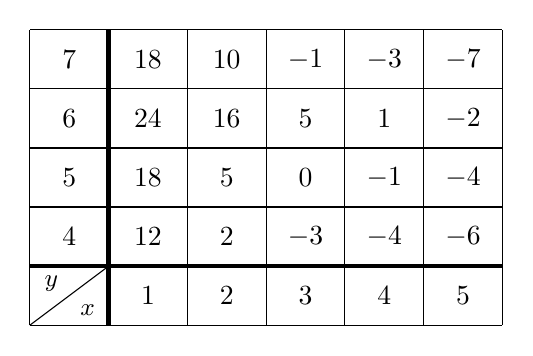
\begin{tikzpicture}[x=1cm,y=.75cm]
        \draw (0,0) grid [step=1] (6,5);
        
        \draw[ultra thick] (0,1)--(6,1);
        \draw[ultra thick] (1,0)--(1,5);
        
        \draw (0,0) -- (1,1);
        \node at (.4,.9) [below left,inner sep=1pt] {\small$y$};
        \node at (0.6,.1) [above right,inner sep=1pt] {\small$x$};
    
        %% y-values
        \node at (0.5,4.5) {$7$};
        \node at (0.5,3.5) {$6$};
        \node at (0.5,2.5) {$5$};
        \node at (0.5,1.5) {$4$};
        
        
        %% z-values
        %% top
        \node at (1.5,4.5) {$18$};
        \node at (2.5,4.5) {$10$};
        \node at (3.5,4.5) {$-1$};
        \node at (4.5,4.5) {$-3$};
        \node at (5.5,4.5) {$-7$};
        
        %% 
        \node at (1.5,3.5) {$24$};
        \node at (2.5,3.5) {$16$};
        \node at (3.5,3.5) {$5$};
        \node at (4.5,3.5) {$1$};
        \node at (5.5,3.5) {$-2$};
        
        %% 
        \node at (1.5,2.5) {$18$};
        \node at (2.5,2.5) {$5$};
        \node at (3.5,2.5) {$0$};
        \node at (4.5,2.5) {$-1$};
        \node at (5.5,2.5) {$-4$};
        
        %% 
        \node at (1.5,1.5) {$12$};
        \node at (2.5,1.5) {$2$};
        \node at (3.5,1.5) {$-3$};
        \node at (4.5,1.5) {$-4$};
        \node at (5.5,1.5) {$-6$};
        
        %% bottom row
        \node at (1.5,.5) {$1$};
        \node at (2.5,.5) {$2$};
        \node at (3.5,.5) {$3$};
        \node at (4.5,.5) {$4$};
        \node at (5.5,.5) {$5$};
      \end{tikzpicture}
    \end{image}
    Estimate $\grad F(3,5)$.
    \begin{explanation}
      We estimate $\grad F(3,5)$ by estimating the partial derivatives. 
      To estimate $F^{(1,0)}(3,5)$, we examine the change in $F(x,5)$
    between $x=4$ and $x=3$:
    \[
    \frac{F(4,5)-F\left(\answer[given]{3},5\right)}{\answer[given]{4}-3}= \answer[given]{-1}
    \]
    We should also examine the change in $F(x,5)$ between $x=3$ and
    $x=2$:
    \[
      \frac{F(3,5)-F\left(\answer[given]{2},5\right)}{\answer[given]{3}-2} =\answer[given]{-5}  
    \]
    Now if we average these values together, we see:
    \[
    \eval{\pp{x} F(x,y)}_{(x,y)=(3,5)} \approx \answer[given]{-3}
    \]
    On the other hand, using a similar procedure, we find that:
    \[
    \eval{\pp{y} F(x,y)}_{(x,y)=(3,5)} \approx \answer[given]{4}
    \]
    Thus the gradient is
    \[
    \grad F(3,5) = \vector{\answer[given]{-3},\answer[given]{4}}
    \]
    Note if you leave the point $(3,5)$ in the direction of $\grad
    F(3,5) = \vector{\answer[given]{-3},\answer[given]{4}}$, you head
    toward $F(2,6)= \answer[given]{16}$, the greatest initial increase
    from $(3,5)$.
    \end{explanation}
\end{example}

\begin{question}
  Here is a plot of an elliptic paraboloid $G(x,y) = x^2 + y^2$ along
  with a vector attached to a point on the surface:
  \begin{image}
    \begin{tikzpicture}
      \begin{axis}%
        [tick label style={font=\scriptsize},axis on top,
	  axis lines=center,
	  view={155}{25},
	  name=myplot,
	  %xtick=\empty,
	  %ytick={5},
	  %ztick={.7,-.7},
	  %minor xtick=1,
	  %minor ytick=1,
	  ymin=-4.4,ymax=4.5,
	  xmin=-4.5,xmax=4.5,
	  zmin=-1.1, zmax=17,
	  every axis x label/.style={at={(axis cs:\pgfkeysvalueof{/pgfplots/xmax},0,0)},xshift=-5pt,yshift=-1pt},
	  xlabel={\scriptsize $x$},
	  every axis y label/.style={at={(axis cs:0,\pgfkeysvalueof{/pgfplots/ymax},0)},xshift=4pt,yshift=-4pt},
	  ylabel={\scriptsize $y$},
	  every axis z label/.style={at={(axis cs:0,0,\pgfkeysvalueof{/pgfplots/zmax})},xshift=0pt,yshift=4pt},
	  zlabel={\scriptsize $z$},colormap/cool
        ]
        \addplot3[domain=-3:3,y domain=-3:3,mesh,samples y=15,very thin,z buffer=sort,%opacity=.6,
          samples=15,] (x,y,{x^2+y^2});
        \addplot3[ultra thick, penColor, ->] coordinates {(-2,2,8) (-3,3,16)};
        \filldraw [black] (axis cs:-2,2,8) circle (2.5pt);        
      \end{axis}
    \end{tikzpicture}
  \end{image}
  True or false: The vector above could be the gradient vector for $G$ at the point.
  \begin{prompt}
  \begin{multipleChoice}
    \choice{True}
    \choice[correct]{False}
  \end{multipleChoice}
  \begin{feedback}
    The answer is ``False.'' Here the graph of the function is three
    dimensional. The gradient vector is in one less dimension than the
    function's graph. Hence the gradient of $G$ is in fact always a
    two dimensional vector.
  \end{feedback}
  \end{prompt}
\end{question}

So far we have mostly talked about the direction of the gradient
vector. Now let's talk about the \textit{magnitude} of the gradient
vector. The magnitude of the gradient vector tells you ``how fast''
the function is increasing.


\begin{question}
  Suppose you have a differentiable function $F:\R^2\to\R$ with the
  following set of level curves.  You should interpolate reasonable
  values of the function $F$ between the level curves which are shown:
  \begin{image}
    \begin{tikzpicture}	
      \draw[ultra thick, penColor] (0,0) ellipse (1.1cm and .8cm);
      \draw[ultra thick, penColor] (.3,0) ellipse (1.5cm and 1cm);
      \draw[ultra thick, penColor] (.7,0) ellipse (2cm and 1.2cm);
      \draw[ultra thick, penColor] (1,0) ellipse (2.4cm and 1.5cm);
      \draw[ultra thick, penColor] (1.3,0) ellipse (2.8cm and 1.8cm);
      \draw[ultra thick, penColor] (1.6,0) ellipse (3.2cm and 2.1cm);

      \node[penColor,fill=white] at (.6,-.6) {\small$7$};
      \node[penColor,fill=white] at (1.2,-.8) {\small$6$};
      \node[penColor,fill=white] at (1.8,-1) {\small$5$};
      \node[penColor,fill=white] at (2.4,-1.2) {\small$4$};
      \node[penColor,fill=white] at (3,-1.4) {\small$3$};
      \node[penColor,fill=white] at (3.6,-1.6) {\small$2$};

      \draw[fill=black,black] (3.7,0) circle (.1cm);
      \draw[fill=black,black] (1.3,1.65) circle (.1cm);
      \draw[fill=black,black] (-1.3,0) circle (.1cm);

      \node[black] at (-2,0) {$B$};
      \node[black] at (.8,2.5) {$A$};
      \node[black,above] at (3.7,0) {$C$};

      \draw[thick,->] (-1.8,0) -- (-1.5,0);
      \draw[thick,->] (.9,2.3) -- (1.2,1.7);
    \end{tikzpicture}
  \end{image}
  Consider the points $A$, $B$, and $C$ on the surface $z=F(x,y)$.
  Where $|\grad F|$ largest?
  \begin{prompt}
    The magnitude of the gradient vector of $F$ is largest at point
    $\answer[format=string]{B}$.
  \end{prompt}
  Where is $|\grad F|$ smallest?
  \begin{prompt}
    The magnitude of the gradient vector of $F$ is smallest at point
    $\answer[format=string]{C}$.
  \end{prompt}
\end{question}




Now, stand back. We're going to do some serious calculus. Just
read, relax and enjoy.

\begin{example}
  Consider the surface given by $F(x,y)= 20-x^2-2y^2$:
  \begin{image}
    \begin{tikzpicture}
      \begin{axis}%
        [tick label style={font=\scriptsize},axis on top,
	  axis lines=center,
	  view={155}{25},
	  name=myplot,
	  %xtick=\empty,
	  %ytick={5},
	  %ztick={.7,-.7},
	  %minor xtick=1,
	  %minor ytick=1,
	  ymin=-1,ymax=5.5,
	  xmin=-1,xmax=5.5,
	  zmin=-1.1, zmax=21,
	  every axis x label/.style={at={(axis cs:\pgfkeysvalueof{/pgfplots/xmax},0,0)},xshift=-5pt,yshift=-1pt},
	  xlabel={\scriptsize $x$},
	  every axis y label/.style={at={(axis cs:0,\pgfkeysvalueof{/pgfplots/ymax},0)},xshift=4pt,yshift=-4pt},
	  ylabel={\scriptsize $y$},
	  every axis z label/.style={at={(axis cs:0,0,\pgfkeysvalueof{/pgfplots/zmax})},xshift=0pt,yshift=4pt},
	  zlabel={\scriptsize $z$},colormap/cool
        ]
        
        %\addplot3[domain=0:180,smooth,y domain=0:360,surf,%fill=white,
        %colormap={mp2}{\colormapplaneone},faceted color=black!40,samples=30,samples y=25,very thin,z buffer=sort] ({cos(x)*1.5*cos(y)},{sin(x)*cos(y)},{sin(y)});
        
        \addplot3[domain=-1:4,y domain=-1:3,mesh,samples y=15,very thin,z buffer=sort,%opacity=.6,
          samples=15,] (x,y,{20-x^2-2*y^2});
        
        \addplot3 [thick, penColor, smooth,domain=1:4,samples=20,samples y=0] ({x},{x^2/4},{20-x^2-0.125*x^4});
        %%        
        \filldraw [black] (axis cs:1,.25,18.875) circle (1pt);
        %\filldraw [black] (axis cs:.5,.25,19.625) circle (1pt);
        %
        %\filldraw [black] (axis cs:.5,.5,19.25) circle (1pt);
        
        
        %\addplot3 [thick,{\colorone}, smooth,domain=-3:3,samples=20,samples y=0] ({x},{2},{x^2+8});
        %
        %\addplot3 [thick,{\colorone}, smooth,domain=-30:170,samples=60,samples y=0] ({2.93*(cos(x))},{1.96*(sin(x))},.2);
        %
        %\addplot3 [thick,{\colorone}, smooth,domain=-30:170,samples=60,samples y=0] ({2.75*(cos(x))},{1.83*(sin(x))},.4);
        %
        %\addplot3 [thick,{\colorone}, smooth,domain=-35:170,samples=60,samples y=0] ({2.4*(cos(x))},{1.6*(sin(x))},.6);
        %
        %\addplot3 [thick,{\colorone}, smooth,domain=-40:170,samples=60,samples y=0] ({1.8*(cos(x))},{1.2*(sin(x))},.8);
        %
        %\filldraw [{\colorone}] (axis cs: 0,0,1) circle (1pt);
      \end{axis}
    \end{tikzpicture}
  \end{image}
  
  Water is poured on the surface at $(1,1/4)$. What path does it take
  as it flows downhill?
  \begin{explanation}
    Let $\vec{w}(t) = \vector{x(t), y(t)}$ be the vector-valued
    function describing the path of the water in the $(x,y)$-plane. We
    seek $x(t)$ and $y(t)$. We know that water will always flow
    downhill in the initial steepest direction. Therefore, at any
    point on its path, it will be moving in the direction of
    \[
    -\grad F(x,y)
    \]
    We'll ignore the physical effects of momentum on the water.  Thus
    $\vec{w}(t)$ will be parallel to $\grad F$. Ah! This means there
    is some constant $c$ such that
    \[
    c\grad F(x(t),y(t)) = \vec{w}'(t) = \vector{x'(t), y'(t)}.
    \]
    Computing the gradient,
    \[
    \grad F(x(t),y(t)) = \vector{-2x(t), -4y(t)}
    \]
    Then
    \begin{align*}
      c\cdot \grad F(x(t),y(t)) &= \vector{ x'(t), y'(t)}\\
      c\cdot \vector{-2x(t),-4y(t)} &= \vector{ x'(t), y'(t)}\\
      \vector{-2cx(t),-4cy(t)} &= \vector{ x'(t), y'(t)}\\
          \end{align*}
    This implies
    \[
    -2cx(t) = x'(t) \quad \text{and} \quad  -4cy(t) =y'(t)
    \]
    so
    \[
    c = -\frac{x'(t)}{2x(t)} \quad \text{and} \quad  c =-\frac{y'(t)}{4y(t)}.
    \]
    Now recall that the differentials $\d x = x'(t) \d t$, and $\d
    y=y'(t)\d t$, so we may write
    \begin{align*}
      \int \frac{1}{2x}x'(t)\d t &=\int \frac{1}{4y} y'(t)\d t \\
      \int \frac{1}{2x}\d x &=\int\frac{1}{4y}\d y \\
      \frac{1}{2}\ln|x| +C &= \frac{1}{4}\ln|y|\\
      2\ln|x| + C &= \ln|y|\\
      \ln|x^2| + C &= \ln|y|
    \end{align*}
    Raising $e$ to the left-hand and right hand sides, we see
    \begin{align*}
    e^{\ln|x^2| + C} &= e^{\ln|y|}\\
    x^2\cdot e^C + C &= \ln|y|,
    \end{align*}
    setting $K = e^C$, we write
    \[
    K\cdot x^2 = y.
    \]
  We are so close to being done, $y=K\cdot x^2$, this is the path
  described in the $(x,y)$-plane. Since the water started at the point
  $(1,1/4)$, we can solve for $K$:
\[
K\cdot 1^2 = \frac14 \quad \Rightarrow \quad K = \frac14.
\]
Thus the water follows the curve
\[
y=x^2/4
\]
in the $(x,y)$-plane.
  \end{explanation}
\end{example}

\begin{question}
  What were you supposed to learn from that last example?
  \begin{prompt}
  \begin{multipleChoice}
    \choice{I've thought about this.}
    \choice{I've not thought about this.}
  \end{multipleChoice}
  The key take-away from the example above is that the negative of the
  gradient points in the initial direction of greatest decrease. The
  other take-away from the example above is just to observe how the
  problem combines many aspects of calculus.
  \end{prompt}
\end{question}







\section{Orthogonality and the gradient}




    LEVEL CURVES MAXIMUM AND ORTHOGONALITY

    IMPLICIT SURFACE GRAPH and VECTORS

Now that we know gradient vectors point in the direction of the
greatest initial increase of the function, let's learn about their
geometry. Consider again a plane. This time we'll think about
\[
z = F(x,y) = x+y
\]
This plane increase with both the $x$-values and $y$-values and passes
through the line $y=-x$ in the $(x,y)$-plane.
\begin{onlineOnly}
\begin{sageCell}
f(x,y) = x+y
plot3d(f, (x,-3,3), (y,-3,3))
\end{sageCell}
\end{onlineOnly}
Let's look at a contour plot:
    \begin{image}
      \begin{tikzpicture}
        \begin{axis}%
          [tick label style={font=\scriptsize},axis on top,
	    axis lines=center,
            width=3in,
            height=3in,
	    xtick={-3,-2,...,3},
            ytick={-3,-2,...,3},
	    %ytick={5},
	    %ztick={.7,-.7},
	    ymin=-1.2,ymax=1.2,
	    xmin=-1.2,xmax=1.2,
            grid=major,%width=3in,height=3in,
            grid style={dashed, gridColor},
	    every axis x label/.style={at={(axis cs:\pgfkeysvalueof{/pgfplots/xmax},0,0)},xshift=5pt,yshift=0pt},
	    xlabel={\scriptsize $x$},
	    every axis y label/.style={at={(axis cs:0,\pgfkeysvalueof{/pgfplots/ymax},0)},xshift=4pt,yshift=2pt},
	    ylabel={\scriptsize $y$},
	  ]
          \addplot[very thick, penColor,smooth] {-x};
          \addplot[very thick, penColor,smooth] {-x+1};
          \addplot[very thick, penColor,smooth] {-x+2};
          \addplot[very thick, penColor,smooth] {-x+3};
          \addplot[very thick, penColor,smooth] {-x-1};
          \addplot[very thick, penColor,smooth] {-x-2};
          
          \node[penColor,fill=white] at (axis cs:.5,-.5) {$0$};
          \node[penColor,fill=white] at (axis cs:0.8,.2) {$1$};
          \node[penColor,fill=white] at (axis cs:1,1) {$2$};
          \node[penColor,fill=white] at (axis cs:-.2,-.8) {$-1$};
          \node[penColor,fill=white] at (axis cs:-1,-1) {$-2$};

          \addplot[color=black,fill=black,only marks,mark=*] coordinates{(4,2)};  %% closed hole          
        \end{axis}
      \end{tikzpicture}
    \end{image}
    Computing the gradient we find
    \[
    \grad F(x,y) = \vector{1,1}
    \]
    This vector is perpendicular to all the level curves.
        \begin{image}
      \begin{tikzpicture}
        \begin{axis}%
          [tick label style={font=\scriptsize},axis on top,
	    axis lines=center,
	    %view={30}{30},
	    %name=myplot,
            width=3in,
            height=3in,
	    xtick={-3,-2,...,3},
            ytick={-3,-2,...,3},
	    %ytick={5},
	    %ztick={.7,-.7},
	    ymin=-1.2,ymax=1.2,
	    xmin=-1.2,xmax=1.2,
            grid=major,%width=3in,height=3in,
            grid style={dashed, gridColor},
	    every axis x label/.style={at={(axis cs:\pgfkeysvalueof{/pgfplots/xmax},0,0)},xshift=5pt,yshift=0pt},
	    xlabel={\scriptsize $x$},
	    every axis y label/.style={at={(axis cs:0,\pgfkeysvalueof{/pgfplots/ymax},0)},xshift=4pt,yshift=2pt},
	    ylabel={\scriptsize $y$},
	  ]
          \addplot[very thick, penColor,smooth] {-x};
          \addplot[very thick, penColor,smooth] {-x+1};
          \addplot[very thick, penColor,smooth] {-x+2};
          \addplot[very thick, penColor,smooth] {-x+3};
          \addplot[very thick, penColor,smooth] {-x-1};
          \addplot[very thick, penColor,smooth] {-x-2};
          
          \node[penColor,fill=white] at (axis cs:.5,-.5) {$0$};
          \node[penColor,fill=white] at (axis cs:0.8,.2) {$1$};
          \node[penColor,fill=white] at (axis cs:1,1) {$2$};
          \node[penColor,fill=white] at (axis cs:-.2,-.8) {$-1$};
          \node[penColor,fill=white] at (axis cs:-1,-1) {$-2$};

          \addplot[penColor2,ultra thick, ->] coordinates{(0,0) (1,1)};

          \addplot[color=black,fill=black,only marks,mark=*] coordinates{(4,2)};  %% closed hole          
        \end{axis}
      \end{tikzpicture}
    \end{image}
    This is \textbf{not} an accident, rather it is a general
    rule. Gradient vectors point in the initial direction of greatest
    increase. \textbf{Every} point on the level curve $1 = x+y$ gives
    the same $z$-value. Because of this if the gradient pointed any
    direction other than, ``directly away,'' and hence
    perpendicularly, from the level curve, it would not be pointing
    in the initial direction of greatest increase. The up-shot?
    \begin{quote}
      \textbf{Gradient vectors are always orthogonal to level
        sets.}
    \end{quote}

    The fact that the gradient is always orthogonal to level surfaces
    is very powerful.  In fact it gives new (easier!) solutions to old
    problems. Let's use this fact to find a plane tangent to a
    surface.
    
    \begin{example}
      Find an implicit equation for the tangent plane to the elliptic
      paraboloid $z = x^2 + y^2$
      \begin{image}
        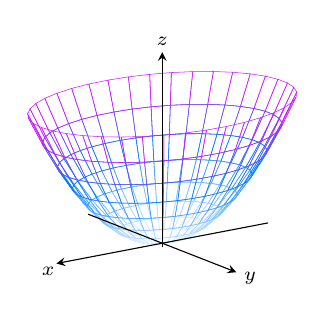
\begin{tikzpicture}
          \begin{axis}%
            [width=175pt,tick label style={font=\scriptsize},axis on top,
	      axis lines=center,
	      view={145}{20},
	      name=myplot,
	      xtick=\empty,
	      ytick=\empty,
	      ztick=\empty,
	      ymin=-2.5,ymax=2.5,
	      xmin=-3.5,xmax=3.5,
	zmin=-.1, zmax=5.5,
	every axis x label/.style={at={(axis cs:\pgfkeysvalueof{/pgfplots/xmax},0,0)},xshift=-3pt,yshift=-3pt},
	xlabel={\scriptsize $x$},
	every axis y label/.style={at={(axis cs:0,\pgfkeysvalueof{/pgfplots/ymax},0)},xshift=5pt,yshift=-2pt},
	ylabel={\scriptsize $y$},
	every axis z label/.style={at={(axis cs:0,0,\pgfkeysvalueof{/pgfplots/zmax})},xshift=0pt,yshift=4pt},
	zlabel={\scriptsize $z$},
        colormap/cool
      ]
            
            \addplot3[domain=0:360,y domain=0:2,color=black!40,mesh,samples=40,samples y=10,very thin,z buffer=sort] ({2*cos(x)*y},{sin(x)*y},{y^2});
          \end{axis}
        \end{tikzpicture}
      \end{image}
      at $\vec{p} = \vector{2,3,13}$.
      \begin{explanation}
        Consider
        \[
        F(x,y,z) =x^2 +y^2 -z
        \]
        and imagine the elliptic parabolid as the level surface
        \[
        F(x,y,z) = \answer[given]{0}
        \]
        Remember, \textbf{the gradient is perpendicular to level
          surfaces}.  We'll use this fact to find a normal vector to
        the surface, and with this vector we'll find the tangent
        plane.  The gradient is:
        \begin{align*}
          \grad F(x,y,z) &= \vector{\pp[F]{x}, \pp[F]{y},\pp[F]{z}}\\
          &= \vector{\answer[given]{2x},\answer[given]{2y}, \answer[given]{-1}}.
        \end{align*}
        Since this vector is normal to the surface, we can use it to
        find an implicit formula for the tangent plane to the surface
        by computing
        \[
        \vec{n}\dotp(\vec{x}-\vec{p}) = 0
        \]
        where $\vec{p} = \vector{2,3,13}$ and
        \begin{align*}
          \vec{n} &= \grad F(\vec{p})\\
          &=\vector{\answer[given]{4}, \answer[given]{6},\answer[given]{-1}}
        \end{align*}
        Thus the equation of the plane tangent to the ellipsoid at
        $\vec{p}$ is:
        \[
        \answer[given]{4}(x-2) + 6(y-3) - (z-\answer[given]{13}) = \answer[given]{0}
        \]
      \end{explanation}
\end{example}



    
Finally, sometimes we are given discrete data that can be
adequately described and approximated by differentiable
functions. In this case, the \textbf{concept} of the gradient will
lead you to success.


\end{document}
